\section{Method}
\label{sec:method}
To generate highly unpredictable numbers I use the fact that predicting the order of action of different threads of execution can be extremely difficult even when the actual hardware is available.
Figure~\ref{fig:TrueRand} illustrates two threads of execution writing different values to the same bit in memory.
When this bit in memory, $Mem_0$, is read at a some point in time, it is not possible to know in advance which value it contains without direct access to the internal hardware of the computer.

\begin{figure}
	\centering
		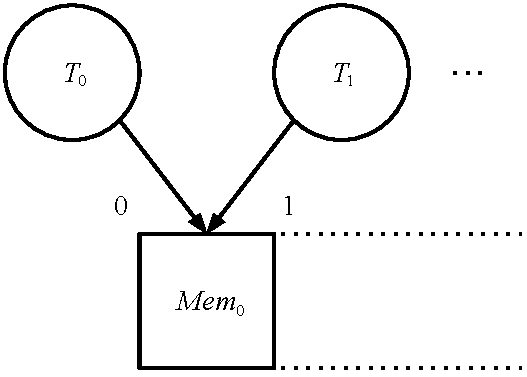
\includegraphics{image/TrueRand.pdf}
	\caption{Two threads of execution writing to the same bit of memory.}
	\label{fig:TrueRand}
\end{figure}

Now that we can construct a single unpredictable bit, the challenge is to expand it to generate larger sequences of memory with unpredictable value.
To accomplish this the first step is simply to add more threads of execution, two to each bit of memory.
Secondly we add a bitmap which indicates whether or not a bit has been touched.
A bit is \emph{touched} when one of the two threads writing to it has actually written something to it.
E.g. $Bitmap_0=0$ until either $T_0$ or $T_1$ has written to $Mem_0$.
When a user of the generator requests a random number, he cannot be served until all the bits in $Mem$ has been touched, i.e. $Bitmap$ contain only 1's.
This technicality is added to ensure that the generator will work even when the random memory block to be generated contains more than half as many bits as there are cores in the processor -- each bit in $Mem$ requires two threads.
If a user is very eager to get many random numbers two requests might be received before some pair of $T$s have had their chance to write to their associated $Mem$.

A considered alternative was to require a predefined time to elapse before the user is served with a number.
This was rejected due to two factors;
First, different computers, OS's, and implementations might behave slightly differently and hence it would require the time to be quite high or risk compromising the quality of the generated random numbers.
Secondly, I aim to allow PMW to run on commodity hardware which means that the workload of the computer can possible change quite dramatic as the user uses his computer for other purposes while random numbers are being generated -- again fording the a pessimistic choice in time limit.
It might be noted that the fact that the user is using his computer might actually increase the entropy much the same way as for the Linux device \texttt{/dev/random}.
Although PMW uses it indirectly as the scheduler of the OS will generally ensure fairness between threads of execution in the long run and the user starts and stops these, thus potentially forcing the scheduler to move other threads (the PMW writing threads in particular) around, possible between physical computation units.

It is important that for all $i\in\left[0..\left|Mem\right|-1\right]:$ $T_{2i}$ and $T_{2i+1}$ are executed on different physical cores.
Otherwise a pattern in the execution of the two threads might give itself away, provided a sufficient number of random numbers are generated.

To test PMW a predefined number of random samples of constant size are requested and the time which it takes to generate these bytes logged.
The throughput of the generator is calculated as the number of samples per time unit.
This throughput is used as comparison to other RNGs.